%!TEX root = thesis_proposal.tex

\chapter{Related work}
\label{chap:rw}

Many relevant research papers have been located and examined as part of the literature review stage of this project. In terms of what was presented in the Research questions section (\ref{chap:rq}), there are two main areas that are of interest: Lidar accuracy (and derived DEM accuracy), and road feature identification in Lidar point clouds. Information about why I will be primarily focusing on a Lidar dataset as the source of elevation measurements can be found in the Tools and datasets (\ref{chap:td}) and Methodology (\ref{chap:m}) sections. The literature review concerning these two areas will be presented below in two separate sections.

\section*{Lidar accuracy}
\label{section:lidaraccuracy}
\subsection*{Accuracy description of Lidar sensing}
\label{subsection:lidarsensingaccuracy}

\begin{wrapfigure}{r}{0.45\textwidth}
    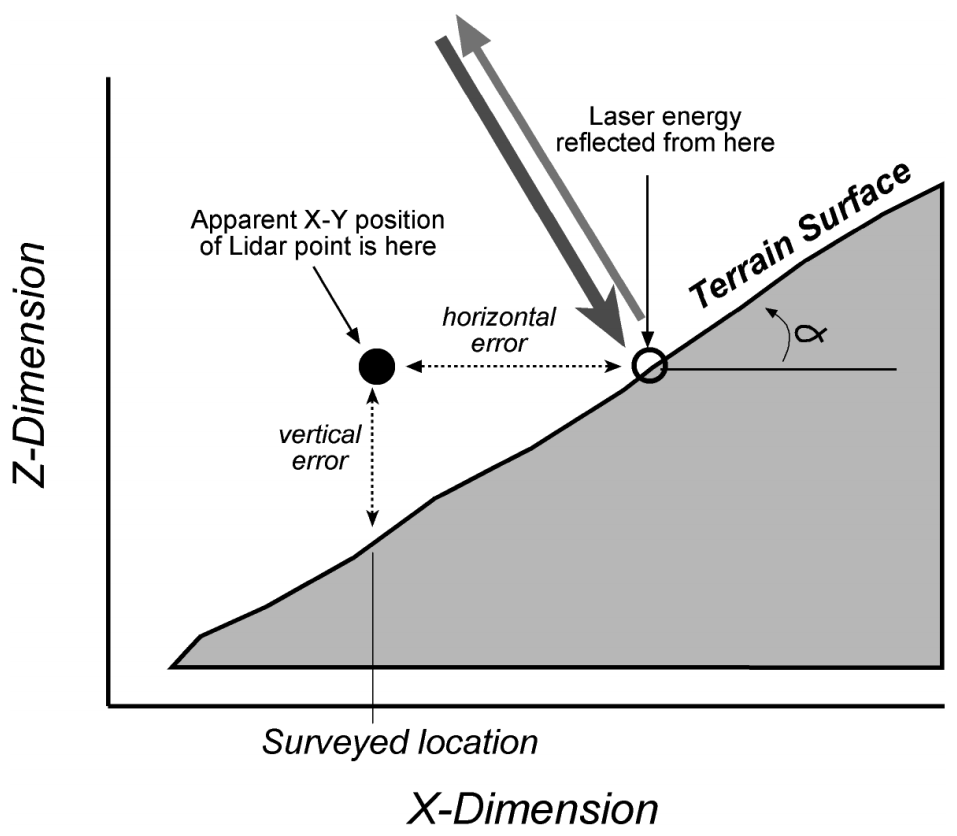
\includegraphics[width=0.95\linewidth]{p2/figs/hodgson_breshanan_2004_01.png} 
    \caption{Sketch diagram showing the effects of horizontal error on vertical accuracy in the context of sloped surfaces. Any uncertainty in the lateral position of the point of reflection will be scaled by the tangent of the slope angle, denoted by \alpha in this diagram (\cite{hodgson_breshanan_2004}).}
    \label{fig:elevationaccuracy}
\end{wrapfigure}

First and foremost, many papers describe that the accuracy of Lidar-derived DEMs depends on the accuracy of the sensing method itself. The notable paper \cite{hodgson_breshanan_2004} describes the most fundamental sensing errors of Lidar measurements to be introduced by Global Navigation Satellite System (GNSS, such as GPS) errors, Inertial Navigation Unit (INS) errors, Inertial Measurement Unit (IMU) errors, errors introduced by the waveform analysis algorithm and lastly, a general error factor that depends on the flying height. Combined, these are the primary factors that contribute to the measurement accuracy of a Lidar survey, together making up the nominal accuracy of a given survey, meaning the figures that can be found in the documentation accompanying Lidar data. Horizontal and vertical accuracy is generally reported separateIt is shown by various research including \cite{hodgson_breshanan_2004}, \cite{su_bork_2006}, \cite{kraus_etal_2006}, \cite{raber_etal_2007}, \cite{peng_shih_2006}, \cite{chow_hodgson_2009}, \cite{aguilar_etal_2005}, \cite{aguilar_etal_2010} \cite{guo_etal_2010} that there are further, local factors influencing Lidar accuracy, which are not related to the sensing equipment and are not generally reported by data providers because they are difficult to estimate and vary spatially. It is widely regarded in the above set of papers that elevation errors increases linearly as a function of increasing topographic complexity (commonly represented as a 2D slope map), and logarithmically as a function of decreasing local point density (falling off rapidly beyond a certain threshold density). Furthermore, an equivocal consensus also exists regarding the influence of vegetation. In all cases it decreases accuracy, with the significance of the error depending strongly on the type of vegetation. Mature trees and evergreens tend to influence accuracy to a lesser extent, whereas bushes, shrubs and undergrowth in general tend to have a decidedly larger impact. \cite{peng_shih_2006} quantified this as a function of \textit{vegetation angle}, a qualitative measure (not a real angle) that describes how well Lidar can theoretically penetrate various types of vegetation. They found that there is a linear correlation between elevation errors and vegetation angle, as well as canopy volume. The one exception is \cite{raber_etal_2007} which reported specifically that in very strongly vegetated areas, no correlation could be found between vegetation classes and accuracy (or even point density and accuracy). Research tackling these topics uses empirical methods to estimate errors, which generally consist of surveying ground control points accurately and either directly comparing with nearby Lidar points, or first constructing a spatially continuous DEM and comparing the interpolated values in the DEM with the surveyed reference elevations. The papers also establish that correlations exist between the examined sources of error, most importantly between vegetation and point density, with the latter intuitively decreasing in places of significant vegetation cover. Other correlations have also been reported, for instance between point spacing and vegetation angle, as well as point spacing and slope in \cite{peng_shih_2006}, and a weak logarithmic correlation between point density and slope by \cite{chow_hodgson_2009}.

The point is made in several of these papers that because of the logarithmic correlation between point spacing and accuracy, increasing the target point density of a survey is only justified up to a certain point. This depends strongly on the study area because point density itself is correlated with the vegetation cover and often the terrain relief. In most of the mentioned papers, the pinpointing of specific sources of error and the type of correlation include traditional methods of manual or automatic 1D or 2D regression, as well as for instance supervised classification with potential sources of errors as the variables. It is argued by several authors, most prominently by \cite{guo_etal_2010}, that in vegetation-free areas of low relief, most ALS surveys oversample the terrain by as much as 30 to 50 percent, leading to increased processing times, reduced algorithmic stability, and no improvement in accuracy. \cite{bater_coops_2009} comes to the same conclusion, and the logarithmic trend generally observed between point density and elevation accuracy further supports this. Conversely, in rugged, vegetation-covered terrain additional cross-flight surveys can increase accuracy significantly by improving ground point density, as \cite{peng_shih_2006} noted.

\subsection*{Accuracy description of Lidar-based DEM-generation}
\label{subsection:lidardemaccuracy}

The topic of the influence of DEM interpolators (specifically, DTM interpolators) on accuracy has also been widely studied. There exist various types of approaches, such as deriving exact error propagation formulae from the mathematical descriptions of certain interpolators, as well as the more popular approaches based on simply performing the interpolation and checking its accuracy post-application via split-sample, cross-validation or jack-knife methods. As an example of the theoretical approach, \cite{aguilar_etal_2010} propagates errors mathematically through the IDW interpolator to obtain a specific expression. Among other things, such a formula depends on the sensing accuracy, the local factors of accuracy (e.g. slope), the gridding resolution, as well as a mathematical expression derived from the interpolator’s formal definition. As that paper shows, it is possible to simplify the process by performing Monte Carlo simulations on the mathematical definition of the interpolator rather than to derive the formula directly. \cite{kraus_etal_2006} also apply a similar, theoretical method to analyse errors propagating through the moving Maximum Likelihood Estimator (MLE). Post-application statistical evaluation was performed by for instance \cite{peng_shih_2006} (jack-knife, using surveyed reference points), and \cite{guo_etal_2010} (ten-fold cross-validation). Notably, \cite{smith_etal_2005} used all three approaches (split-sample, cross-validation, and jack-knife) for a wide range of interpolators in an urban setting.
Firstly, many of these papers examined the influence of gridded DTM resolution on accuracy. \cite{chow_hodgson_2009} examined via regression techniques (on IDW interpolation) how it is correlated with point density and found that linear to logarithmic correlations exist. \cite{guo_etal_2010} argues that for most interpolators, the overall trend is linear between accuracy and resolution, up to the scale of the Lidar point density. They also found that differences in accuracy between interpolators were most prominent at the finest resolution. \cite{bater_coops_2009} found that the local influence on accuracy of slope and point density are mostly invariant relative to DTM resolution. In terms of the accuracy ranking of interpolators, there is a clear consensus that no such ranking exists that is independent of the size and type of the study area, and the purpose of the interpolation. For instance, the accuracy of piecewise spline-based, quintic-type, kriging and ANUDEM methods were found lacking in the context of their insensitivity to small, sudden changes (such as natural faults in the terrain and anthropogenic modifications thereof) while they were proven to work well for large-scale terrain, as described by \cite{bater_coops_2009} and \cite{guo_etal_2010} for instance. All reviewed papers agreed that the accuracy of all interpolators decreases the most in areas of high relief and reduced point density, with spline-based, IDW methods generally producing the worst results in such areas, especially for large-scale terrain. Interestingly, the relative importance of interpolation-introduced errors is reportedly low relative to instrument-related errors and surface-related local sources of error, according to research such as \cite{hodgson_breshanan_2004} and \cite{aguilar_etal_2010}. The former goes as far as to state that the decrease in accuracy after the application of an interpolator is insignificant, or that interpolation may even increase the overall accuracy, although this was observed in densely vegetated areas where point spacing and accuracy are severely afflicted. TIN-based interpolation methods were recommended specifically by \cite{bater_coops_2009} for complex geometries and found it in their research to be the most conservative in terms of RMSE analysis. \cite{hodgson_breshanan_2004} also used TIN-based interpolation in their research, and detected no significant decrease in accuracy following interpolation. Furthermore, \cite{peng_shih_2006} used TIN-based interpolation in their research, in which they found local influences on elevation accuracy highly predictable. Unlike most papers, \cite{aguilar_etal_2010} considers the accuracy of ground filtering explicitly, and states that its success is a precondition of accurate terrain interpolation wherever the terrain is occluded or shaded partially. It suggests the estimation of ground filtering error (even if only from generic values) and its inclusion in overall elevation accuracy. Overall, it is evident from the review (and specifically recommended by various authors) that testing several candidate interpolators before making a final choice is recommended.

\section*{Road identification in point clouds}
\label{section:roadidentification}
\subsection*{Research using point clouds only}
\label{subsection:roadidentificationpconly}

Our second domain of interest is feature extraction because our intention is to not only systematically query a DEM for elevations around the NWB road centrelines, but to take into account the entire road surface as represented by the point cloud. This requires one to identify, or at least approximate which point cloud points were reflected from the surface of the given road.

In terms of point cloud feature extraction techniques relevant to roads, I have looked at a range of papers that give account of a spectrum of divergent methods. One strategy, most prominently represented by \cite{hu_2003} and \cite{hu_etal_2004}, \cite{zhu_mordohai_2009}, \cite{zhu_hyppa_2014}, and \cite{lin_etal_2015} is based on the idea of transitioning to a photogrammetric analysis at some point in the process. First, a set of pre-processing techniques to better characterise potential road points in the source Lidar data are applied, generally by performing some form of filtering (in some cases simply by setting thresholds applicable to returns from bitumen), or by extracting ground planes using various techniques and selecting points that lie close to them. Then, images are rendered from the point cloud from various angles, often using colour-coding based on point properties, and applying photogrammetric methods to identify roads. Sometimes high-definition aerial or satellite imagery is incorporated in the photogrammetric workflows. The success rates of such strategies are mediocre, rely strongly on manual parametrisation, and are unsuitable for large study areas with inhomogeneous types and distribution of roads, as also concluded by the literature review in the paper \cite{yang_etal_2013}.

There is a further widely adapted set of strategies that rely (partly on entirely) on road edge detection. \cite{vosselman_zhou_2009}, \cite{zhang_2010}, \cite{yang_etal_2013} are examples of such research. \cite{vosselman_zhou_2009} presents a method in which a DTM is generated, points close to it are selected in the point cloud, and small, curb-like jumps in elevation are algorithmically detected. The curb points are selected, and a feature extraction method (RANSAC in this case) is used to construct 3D lines from them. Gaps in the lines are closed algorithmically, and B-splines are fitted to optimise the shapes of the road edges. In \cite{zhang_2010}, road cross-sections are inspected in 1D, and the points representing the road surface, the curbs and non-road surfaces are identified. In \cite{yang_etal_2013} an approach is presented in which first cross-sections are identified, ground points are filtered in 1D, and curbs are then identified in the 1D series of ground points. Their approach is unique because it uses moving window (i.e. convolution) methods on the 1D sections to extract the curbs, testing a subset of the points in each iteration to see whether they satisfy a range of rules. While the results of these methods are more flexible, more accurate and more complete in general than the photogrammetric methods, they are not, in their original form, well suited for this project. The cross-section based approach was originally developed for MLS data, where the data is either natively output in the form of road cross-sections (car-mounted front facing sensor), or can be easily extracted from the point cloud in such a form. \cite{vosselman_zhou_2009} is an exception, which demonstrates that a relatively simple approach can be used to detect curbs without the need for native cross-sections in the data. However, a deeper issue undermines our confidence in the applicability of curb-detection methods. Working with a national dataset and focusing on large roads (including motorways) means that the assumption that well-defined, relatively uniform road curbs will exist and be reliably detectable everywhere is not a sensible assumption.

\subsection*{Methods using input point clouds and external vector data}
\label{subsection:roadidentificatiovectordata}

\begin{wrapfigure}{l}{0.45\textwidth}
    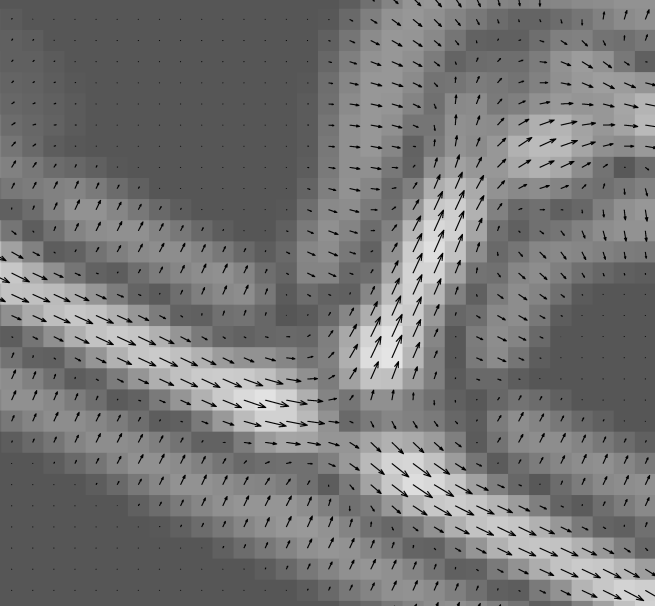
\includegraphics[width=\linewidth]{p2/figs/clode_etal_2007_01.png} 
    \caption{The results of convolution with the Phase Coded Disk (PCD) are illustrated. The vector magnitude in any given pixel quantifies the support that exists there for the presence of a road centreline. It is effectively a centreline detector. Convolving the PCD is in fact a photogrammetric method, hence a binary map is generated from the classified point cloud prior to its application. Nevertheless, the method is still more relevant to us than the rest of the photogrammetry-based research mentioned (\cite{clode_etal_2007}).}
    \label{fig:phasecodeddisk}
\end{wrapfigure}

The remaining selection of methods can be grouped into two categories: ones that use external data as initial approximations of the location of roads, and ones that use point cloud data exclusively.  Examples of the latter are \cite{clode_etal_2004} and \cite{clode_etal_2007}, in which a DEM is generated, points close to the DTM are selected, further filtered based on intensity thresholds applicable to bitumen in a hierarchical system, and then refining the results via morphological operations on the selected regions – resulting in classified road points. In the above 2007 paper, they extend the procedure by convolving the results with a Phase Coded Disk (PCD), which can create a spatial map of the predicted road parameters wherever it moves through road points. They describe it as an alternative to using the Hough-transform for finding road centrelines, which, according to their research, is not reliable enough in this context. This spatial map can then be used to generate a vector dataset describing the geometry of the roads. \cite{gross_thoennessen_2006} shows that point neighbourhood information can be used to generate covariance matrices of individual points, which can in turn be used to decide directly whether the point belongs to a linear feature. They also describe how lines can be assembled from the selected points efficiently. Other methods relying only on the points themselves exist, but they are typical of real-time MLS applications, such as the fully convolutional neural network-based solution in \cite{caltagirone_etal_2017}. The literature review in \cite{yang_etal_2013} offers an excellent overview of such additional methods, but they will not be described here any further, as they are not relevant enough to this project.

\begin{figure}
    \centering
    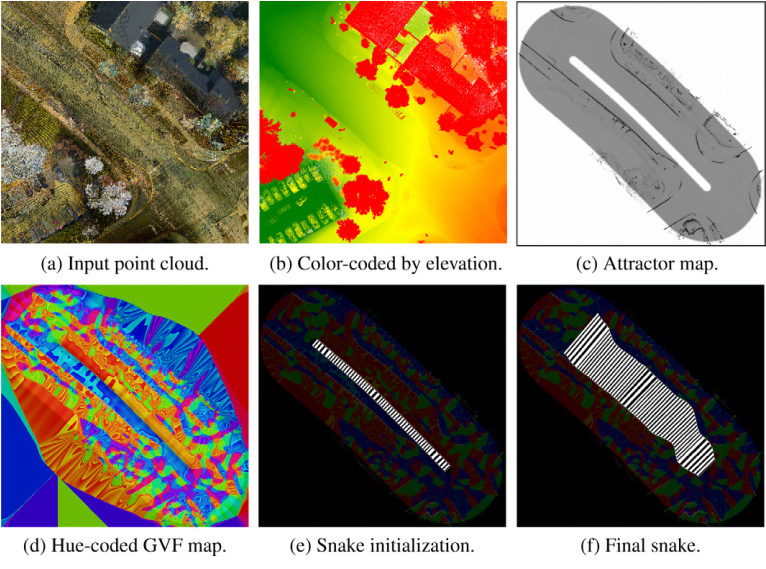
\includegraphics[width=0.75\linewidth]{p2/figs/boyko_funkahuser_2011_01.png} 
    \caption{Illustration of the procedure used in \cite{boyko_funkhauser_2011}, taken from their paper. In the attractor map, darker colours represent stronger attraction, resulting in the active contour converging to them in the optimisation procedure. The GVF map is a vector map that contributes to favourable active contour convergence and is not described any further here. The initial contour is based on the road centreline (from external vector data).}
    \label{fig:activecontouroptimisation}
\end{figure}

The last category contains research that used similar input data to ours (including initial road estimate vector datasets) and achieved similar goals. \cite{cai_rasdorf_2008} show that enriching road centrelines with elevations can be achieved using simplistic methods. Their first method is based on finding points on opposite sides of the road (in 2D) at similar distances from it, and in suitable locations to form approximate cross-sections. The road is intersected with the cross-section and the intersection is given an elevation by 1D-interpolating inside the cross-section, using the elevations of the two points defining the cross-section. Their second method is even simpler; for each road vertex  (or some sampling along its length), they locate the closest Lidar point and associate its elevation with it. The simplicity of these methods is reminiscent of the commercial solutions which were developed for NDW by RHDHV (described in the Methodology section), and highlights that a rough approximation for the road elevations can, in practice, be made either directly from the point cloud or from a derived DTM in a straightforward manner. However, far more sophisticated methods have been developed by other authors. One landmark research, \cite{boyko_funkhauser_2011}, describes a method in which their input polylines are used to label road points in an ALS point cloud. They first associate the input lines with elevations by fitting spline curves through nearby Lidar points. Suitable Lidar points are selected based on minimising an error function that includes terms related to the distance from the location of interpolation, and to elevation variance. The resulting network is guaranteed to be continuous and smooth because the densified input polylines are used as a spline control points. They then partition the point cloud on disk, based on fitting small support planes along the 3D-converted lines and fetching points that are close to them (solving both the memory and the 2.5D violations related to overlapping roads). They then construct an attractor map penalising points away from road edges based on one term depending on the distance from the road centreline, and another based on a curb detection algorithm. Lastly, they apply an active contour (snake) optimisation technique that yields the road edges in 3D, and then label points between the two edges as road points. An illustration is shown in Figure \ref{fig:activecontouroptimisation}. \cite{gopfert_etal_2011} demonstrates that such active contours can be used to estimate road outlines without the need for the involved pre-processing steps in \cite{boyko_funkhauser_2011}, simply by taking elevations of the input polylines from a derived DTM and optimising the road centreline the same way as its outline (using the active contours). \cite{hatger_brenner_2003} presents two approaches based on region-growing. The first one is based on growing planes in the entire study area from Lidar points. This being too complex computationally. They propose another approach of treating Lidar scan lines individually, partitioning each into parametrised line segments via linear regression and then inspecting the succession of scan lines and identifying neighbouring segments that are roughly parallel. The resulting groups of (roughly parallel) lines are then treated as planar regions, and an additional region growing step is performed to find any points that might have been left out. The results of this can then either be prepared as a full, 3D-polygon-based planar partition of the study area onto which road polylines can simply be projected, or by further refining the planar partition (eliminating small, meaningless planes) via a RANSAC-based workflow.
\begin{wrapfigure}{r}{0.45\textwidth}
    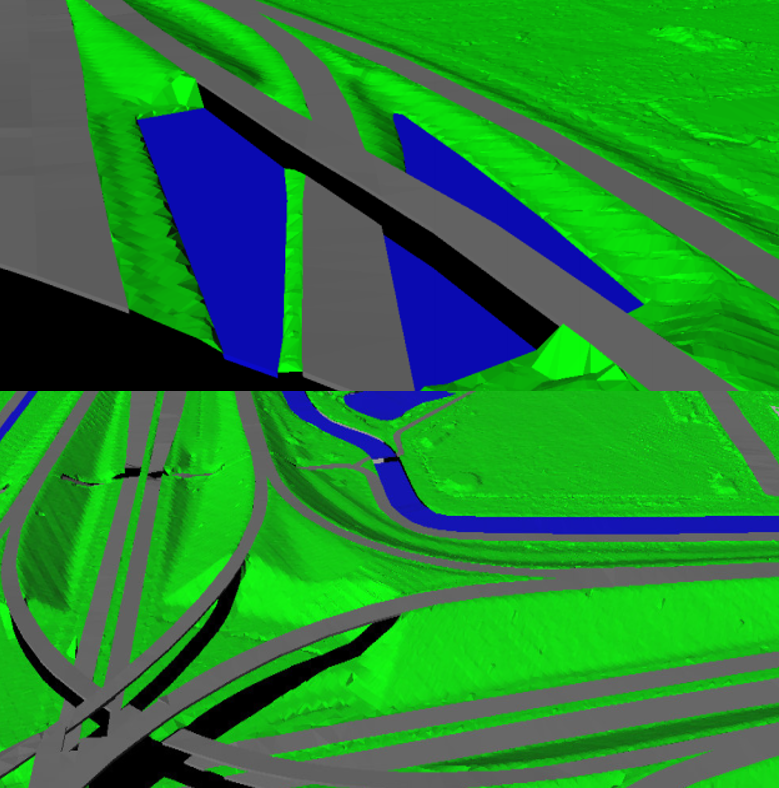
\includegraphics[width=\linewidth]{p2/figs/oudeElberink_vosselman_2006_03.png} 
    \caption{Examples of 3D-converted multi-level road vector geometry showing artefacts that are typical in the context of Lidar point cloud to 3D vector geometry conversion. Most notably, in multi-level configurations of roads, only the one with the highest elevation is converted to 3D (\cite{oudeElberink_vosselman_2006}).}
    \label{fig:conversionartefacts}
\end{wrapfigure}
\cite{oudeElberink_vosselman_2006} is relevant not only because of the methods it applies, but also the datasets. They enrich the best-known Dutch open data national topographical vector dataset (the present-day equivalent of which is BGT) with elevations, and as their source of elevations, they use AHN data. They do not exclusively consider roads; all polygonal vector objects are “extruded” to 3D. Like \cite{hatger_brenner_2003}, they propose region growing as the foundation of the elevation extraction workflow. They use the Hough transform to find seed points whose neighbourhood suggest a planar structure, fit planes and then grow by checking the point-to-plane distance of new points, labelling points with the identifier of the plane they belong to. The vector data is then overlayed, and for each polygon the plane is selected which is represented by the most labelled points in its interior. These points are re-fitted a plane, and each such plane is used to extrude the corresponding overlayed vector geometry simply by projecting onto its surface. To improve upon the results of this simple extrusion, they suggest the application of algorithmic topological corrections. Furthermore, to model the interior of the extruded polygons in more detail, they recommend the construction of a Constrained Delaunay Triangulation (CDT) for each, first by inserting its edges as constraints, and the by inserting the Lidar points that generated its surface. The CDT can be refined algorithmically to ensure smoothness. The main limitation of their method is that its method to extract elevations (the growing approach) is not too accurate, and that it cannot handle overlapping objects, such as roads in motorway interchanges. Their method was later extended in \cite{oudeElberink_vosselman_2009} to work well in complex multi-level road settings by using point cloud segmentation in a manner resembling what I already described in the context of \cite{boyko_funkhauser_2011}. In his doctoral thesis \cite{oudeElberink_2010} he combined this method with the overall procedure in \cite{oudeElberink_vosselman_2006} to form one integral whole. Furthermore he extended it with a road extraction quality assessment procedure, which was later perfected and also published separately in \cite{oudeElberink_vosselman_2012}. Their quality and accuracy assessment methodology is comprised of two separate procedures and the comparison of their results: a theoretical (functional and stochastic) evaluation, and an empirical one against reference data. Interestingly, their reference data was DTB and in general, showed good agreement with their road extraction results.

While none of the above research provides an all-in-one solution to answering the research questions of this project, they contain procedures and concepts which can be used as building blocks for my methodology. The main area \textit{not} explicitly covered by the examined papers is the use of external 3D vector data (DTB in our case) as a further constraint when extracting roads from point clouds. However, methods to perform this can be derived from the operations in them that relate to using vector geometries as approximate road locations in 2D, and from general geomatics concepts and methods. An additional consideration related to the input road centrelines is that in all research presented above, refining the lateral position of the road is permitted. However, NDW specifically requested that I do not move the NWB lines horizontally. Hence, I plan to focus primarily on enriching NWB with elevations without moving them laterally, with only exploring its lateral refinement to a limited extent.